%%%%% slides template
% Giovanni Ramirez (ramirez@ecfm.usac.edu.gt)
% 20200828
% Require: images/ecfmByN.png images/usacByN.jpg
%
%
% Use this option to print notes only
% \documentclass[xcolor=dvipsnames,handout,notes=only]{beamer}%
%
% Use this option to print notes and slides
% \documentclass[xcolor=dvipsnames,handout,notes=show]{beamer}%
%
% Use this option to get a printer-friendly version
% \documentclass[xcolor=dvipsnames,handout]{beamer}%
%
% Unse this option to get slides only
\documentclass[xcolor=dvipsnames,presentation]{beamer}%
%
%%%%%


%%%%% theme and coloring
% a list of themes can be found here https://hartwork.org/beamer-theme-matrix/
% I like a simple Malmoe with some modifications and color-schemes like
% dolphin for a white background, beetle for a gray background or dove for
% plain slides
%
% theme definition
\usetheme{Malmoe}
%
% definition of the presentation mode: full slides
\mode<presentation> {
% coloring for slides other options: beetle, dove
  \usecolortheme{dolphin}
% to include a slide with the table of contents
 \AtBeginSection[] {
  \begin{frame}
    \tableofcontents[currentsection]
  \end{frame} }
}
%
% definition of the handout mode: printer-friendly
\mode<handout>{
% coloring: dove is white
  \usecolortheme{dove}
% this is to print 2 slides in 1 page, other values are allowed
  \usepackage{pgfpages}
  \renewcommand\textbullet{\ensuremath{\bullet}}
  \pgfpagesuselayout{2 on 1}[letterpaper,border shrink=5mm]
% set the fontsize of the notes
  \setbeamerfont{note page}{size=\scriptsize}
% disable the slide with the table of contents
  \AtBeginSection[]{}
}
%%%%%

%%%%% personalisation
% clear all headers
\setbeamertemplate{headline}{}
% disable navigation buttons
\setbeamertemplate{navigation symbols}{}
% configure the blocks used for equations, theorems, etc
\setbeamertemplate{blocks}[rounded][shadow=true]
% clear the footline
\setbeamertemplate{footline}{}
% set the footline
\setbeamertemplate{footline}{
  \hbox{%
% left block with the shortname, it is set in the \author command
    \begin{beamercolorbox}[wd=.40\paperwidth,ht=2.25ex,dp=1ex,center]%
      {author in head/foot}%
      \usebeamerfont{author in head/foot}\insertshortauthor
    \end{beamercolorbox}%
% center block with the short title, it is set in the \title command
    \begin{beamercolorbox}[wd=.50\paperwidth,ht=2.25ex,dp=1ex,center]%
      {title in head/foot}%
      \usebeamerfont{title in head/foot}\insertshorttitle
    \end{beamercolorbox}%
% right block with the number of slides
    \begin{beamercolorbox}[wd=.10\paperwidth,ht=2.25ex,dp=1ex,right]%
      {date in head/foot}%
      \usebeamerfont{date in head/foot}
      \insertframenumber{} / \inserttotalframenumber\hspace*{1em}
    \end{beamercolorbox}}%
  \vskip0pt%
}
%%%%%

%%%%% packages
%
% language, decimal point mark
\usepackage[spanish,es-nodecimaldot]{babel}%
%
% to use only T1 scalable fonts
\usepackage[T1]{fontenc}%
\let\Tiny=\tiny% this is a proper configuration of the tiny font size
%
% to use UTF coding, other options latin1
\usepackage[utf8]{inputenc}%
%
\usepackage{array}
% special math symbols
\usepackage{latexsym,amsfonts,amsmath}%
%
% to include graphics
\usepackage{graphicx}%
% path to images
\graphicspath{ {./img/presentacion/} }
%
% to use tiks: nice to draw diagrams
\usepackage{tikz}%
\usetikzlibrary{arrows,shapes,positioning}
%
% to use SI units and physics notation
\usepackage{physics}%
\usepackage{multirow}
\usepackage{xcolor}
\usepackage{subcaption}
%
% to use hypenation
\usepackage{ragged2e}%
\let\raggedright=\RaggedRight%
%





\usepackage{dsfont}
\usepackage[author={Max Schlepzig}]{pdfcomment}






\newcommand{\subind}[2]{{}_{#1}^{#2}}
%%%%% Talk data
%
%title
\title[Canales cuánticos PCE]% this is the short title
{Mapeos proyectivos en sistemas de varios qubits}% this is the long title
\subtitle{\bf Operaciones PCE \newline\vspace{1.4cm}}
%
% author
\author[José Alfredo de León]% this is the short name
{José Alfredo de León}% this is the long name
%
% affiliation
\institute{Asesorado por:\\Dr. Carlos Francisco Pineda Zorrilla (IFUNAM)
\newline y M.Sc. Juan Diego Chang (ECFM-USAC)}%
%
% date and information about the conference
\date{Miércoles 27 octubre 2021}
%%%%%


%%%%%
\makeatletter
\newenvironment{myitemize}{%
   \setlength{\topsep}{0pt}
   \setlength{\partopsep}{0pt}
   \renewcommand*{\@listi}{\leftmargin\leftmargini \parsep\z@ \topsep\z@ \itemsep\z@}
   \let\@listI\@listi
   \itemize
}{\enditemize}
\makeatother 


\begin{document}
% % % % % % % % % % % % % % % % % % % % % % % % % % % % % % % % % % % % % %
% Title and Outline
% % % % % % % % % % % % % % % % % % % % % % % % % % % % % % % % % % % % % %
\begin{frame}[plain]
  \titlepage 
  \begin{tikzpicture}[x=1mm,y=1mm,overlay,remember picture]
    \pgftransformshift{\pgfpointanchor{current page}{center}}
    \node[inner sep=0pt] (usac) at (-45,-14.5) %
    {
\includegraphics[height=14mm]{logos/ecfmByN}};
    \node[inner sep=0pt] (usac) at (44,-14.5) %
    {
\includegraphics[height=14mm]{logos/ifunam}};
    \node[inner sep=0pt] (usac) at (0,11) %
    {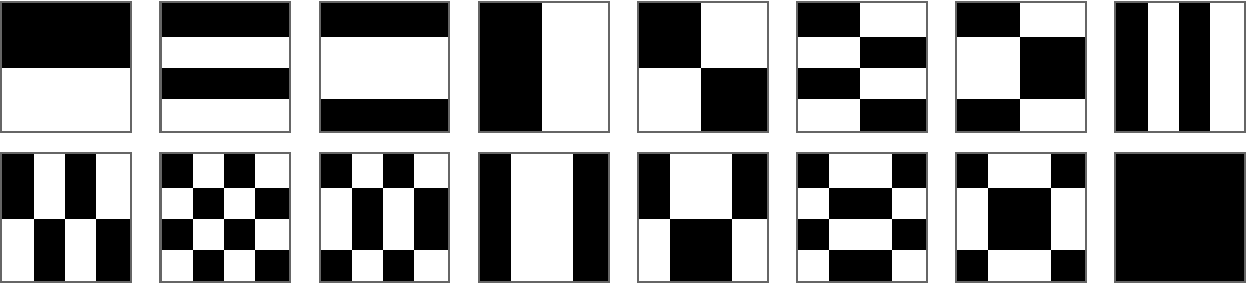
\includegraphics[height=14mm]{portada}};
  \end{tikzpicture}
\end{frame}

\begin{frame}{Agradecimientos}
	\begin{itemize}
		\item A mi familia. En especial, a mi mamá.
		\item A mis asesores: Carlos y Juan Diego. 
		\item A Alejandro Fonseca y David Dávalos.
		\item Al Ingeniero Rodolfo Samayoa.
		\item A mis prefesores de la ECFM.
		\item A Cindy.
		\item A mis amigos Benja, Gómez, Papaya y José Guillermo.
		\item A mis amigos de la U.
	\end{itemize}
\end{frame}

\begin{frame}{Plan de la presentación}
  \tableofcontents 
\end{frame}


% % % % % % % % % % % % % % % % % % % % % % % % % % % % % % % % % % % % % %
% Introduction and Motivation
% % % % % % % % % % % % % % % % % % % % % % % % % % % % % % % % % % % % % %
\section{Introducción}
\label{sec:Intro}
\begin{frame}[t]{Motivación}
	Con frecuencia, una descripción más precisa de un sistema
	cuántico requiere incluir la interacción con su entorno, i.e. 
	considerar al sistema como abierto.
	\begin{columns}
	\column{.5\textwidth}
		\begin{figure}
%		\includegraphics<1>[width=\textwidth]{H_alone}
		\includegraphics<1->[width=\textwidth]{H_w_photons}
		\end{figure}
	\column{.5\textwidth}
		\begin{figure}
%		\includegraphics<1>[width=\textwidth]{lattice}
		\includegraphics<1->[width=\textwidth]{lattice_sub}
		\end{figure}
	\end{columns}
	
	\vfill\alert{En general,
	$\ket{\psi}\ne\ket{\text{sistema principal}}\otimes\ket{\text{entorno}}$}
\end{frame}

\begin{frame}{Motivación}
	Los sistemas abiertos están sujetos a fenómenos de decoherencia.
	\begin{itemize}
	\item Debido al acople con un baño térmico el estado $\ket{\psi}$ 
	colapsa a alguno de los eigenestados $\ket{+}$ o $\ket{-}$, perdiendo 
	así información sobre el estado inicial $\ket{\psi}$ del sistema.

  \item Depolarizante: proceso mediante el cual los estados puros se 
  transforman en estados mixtos.
	\end{itemize}\vfill
	
	Nuestro interés: ¿cómo generalizar estos procesos de decoherencia 
	para sistemas de muchas partículas de 2 niveles utilizando el formalismo
	de los canales cuánticos?
%	\begin{figure}
%	\centering
%	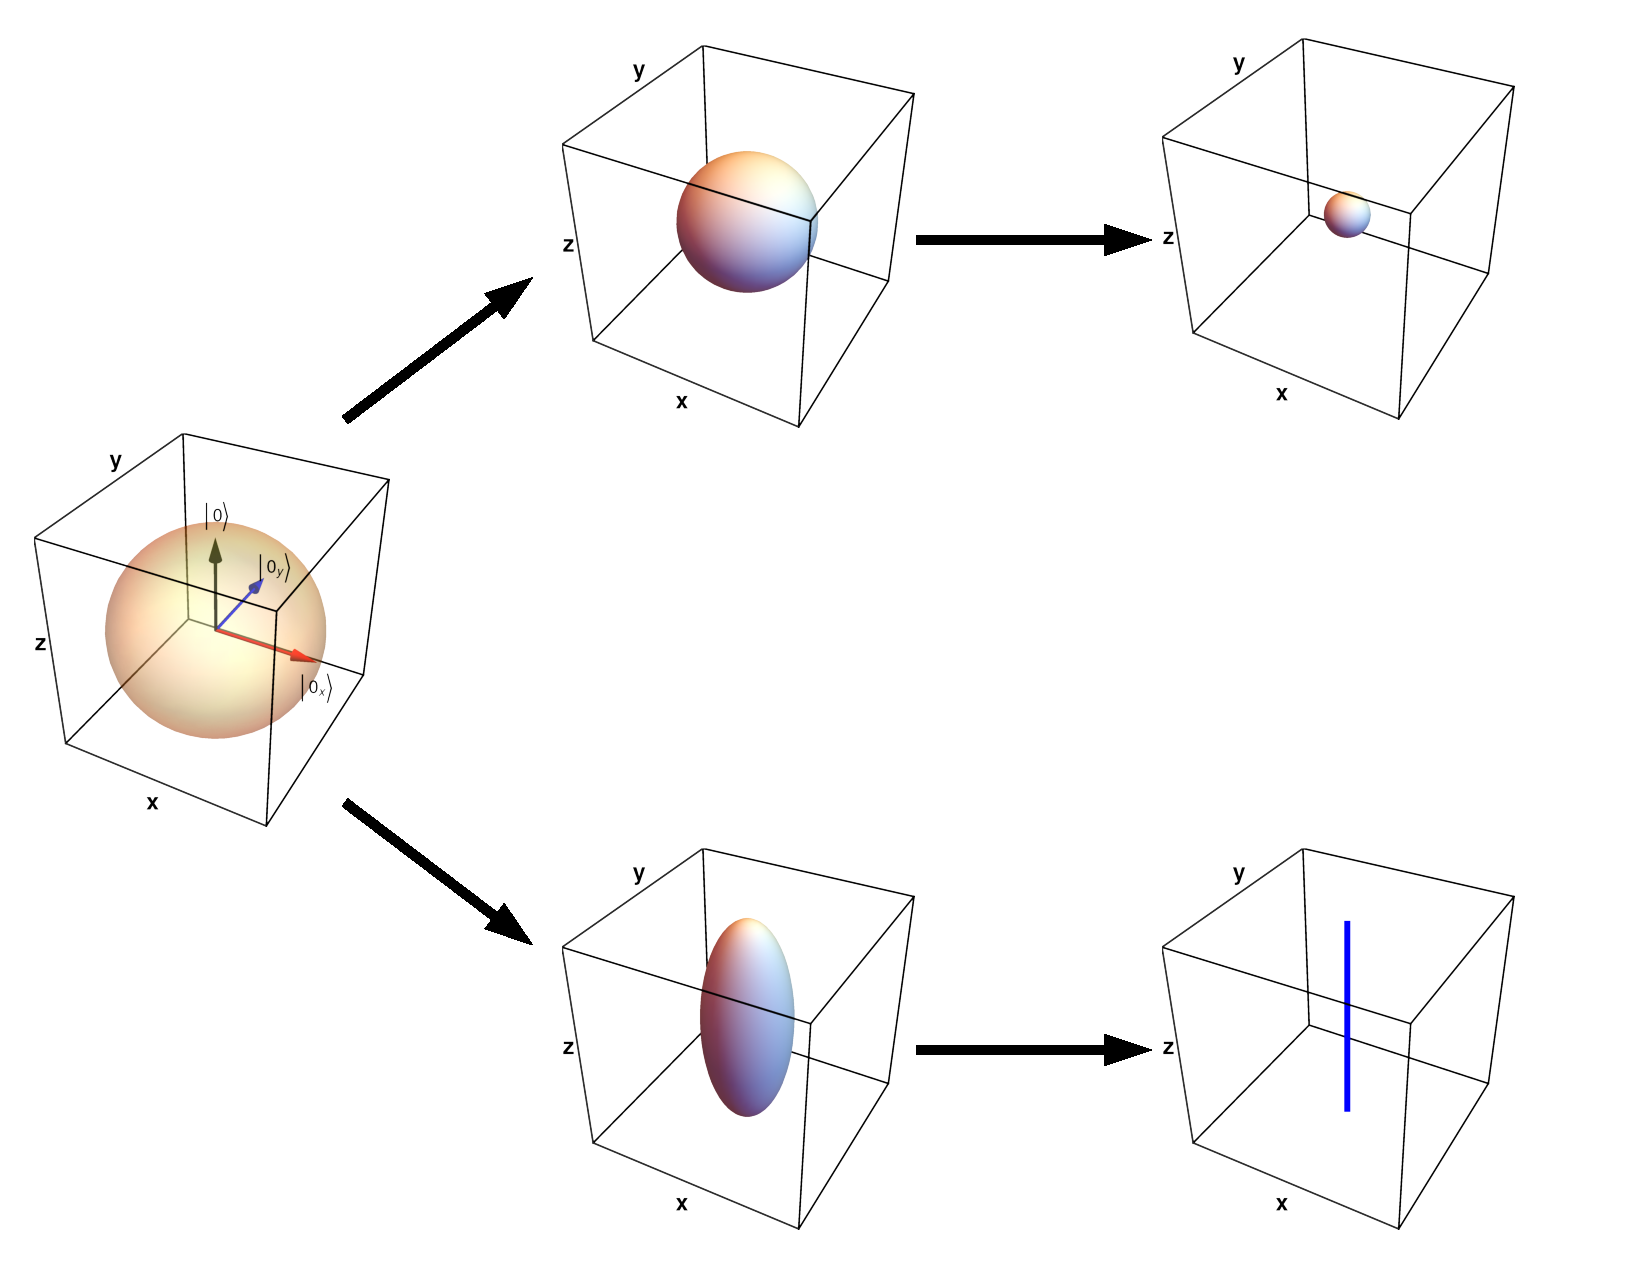
\includegraphics[width=9cm]{decoherencia_motivacion}	
%	\end{figure}
%	 \begin{tikzpicture}[x=1mm,y=1mm,overlay,remember picture]
%    \pgftransformshift{\pgfpointanchor{current page}{center}}
%    \node[inner sep=0pt] (usac) at (35,-2) %
%    {\textcolor{red}{¿cómo describir}};
%    \node[inner sep=0pt] (usac) at (35,-5.5) %
%    {\textcolor{red}{este tipo de procesos?}};
%  \end{tikzpicture}
\end{frame}


\section{Fundamentos teóricos}
\begin{frame}{Matriz  densidad}
Una matriz $\rho$ es una matriz densidad si y sólo si
	\begin{enumerate}
		\item $\Tr (\rho)=1$,
		\item $\matrixel{x}{\rho}{x}\geq 0, \forall \ket{x} \in \mathcal{H}.$
	\end{enumerate}	\vfill

	En el caso particular cuando el sistema se encuentra en un estado
	puro $\ket{\psi}$, la matriz de densidad $\rho$ se escribe
  \begin{align*}
  \rho=\dyad{\psi}{\psi}.
  \end{align*}
\end{frame}

\begin{frame}{Qubits}
Un sistema cuántico de dos niveles recibe el nombre de qubit. \vfill

	\begin{columns}	\hspace{.4cm}
	\begin{column}{0.6\textwidth}
	\begin{itemize}
		\item 1 qubit:
		\begin{align*}
			\rho &= \frac{\mathds{1}+r_1\sigma_x+r_2\sigma_y+r_3\sigma_z}{2}.
		\end{align*}	
		\item $n$ qubits:
		\begin{align*}
		\rho = \frac{1}{2^n}\sum _{j_1,\ldots,j_n=0}^3 r_{j_1,\ldots,j_n}\cdot
		\sigma_{j_1}\otimes \ldots
		\otimes\sigma_{j_n},%\qquad r_{0,\ldots,0}=1,
		\end{align*}
		$r_{j_1,\ldots,j_n}$ componentes de Pauli.
	\end{itemize} \vfill
	\end{column}%\hspace{-1cm}
	\begin{column}{0.4\textwidth}  
  		\begin{center}
    		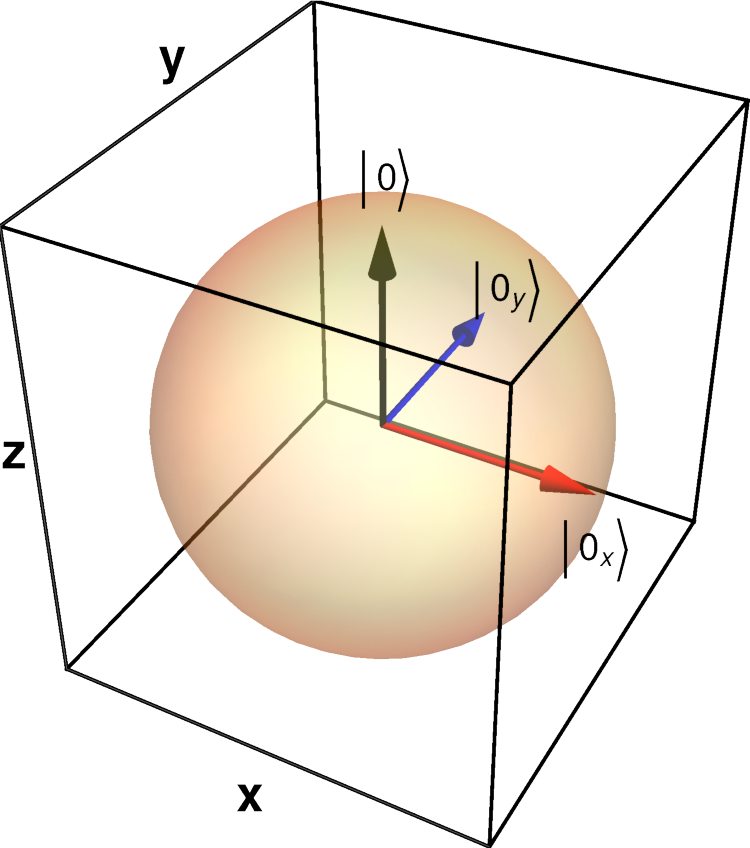
\includegraphics[width=.85\textwidth]{bloch_sphere}      
     \end{center}
		\end{column}
	\end{columns}
\end{frame}

\begin{frame}{Canales cuánticos}%
  %{¿cómo describir la dinámica de los sistemas abiertos?}
  \vfill
  \begin{itemize}
  	\item La teoría de los canales cuánticos es un formalismo para describir 
  la evolución de los sistemas abiertos,
  \begin{align*}
	\mathcal{E}(\rho)=\rho'.
	\end{align*} \vfill
  \only<1>{\item Una operación lineal $\mathcal{E}$ es un canal cuántico 
  si y sólo si
	\begin{enumerate}
	\item Preserva las características de la matriz densidad
	\item Es una operación completamente positiva. Esta condición
	implica que la extensión de un canal $\mathcal{E}$
	$$
	\mathcal{E}\mapsto\qty(\mathcal{E}\otimes \mathds{1}_k)
%	\qty(\mathcal{E}\otimes \mathds{1})\qty[\dyad{\text{Bell}}{\text{Bell}}]\geq 0.
	$$
	debe mapear también matrices densidad en matrices densidad.
	\end{enumerate} \vfill
	} 
  \end{itemize}

\end{frame}	


\begin{frame}{Canales cuánticos de 1 qubit}
	Rotaciones de la esfera de Bloch
	\begin{center}
	\begin{tabular}{m{2.5cm} m{1.8cm} m{2.5cm}}
		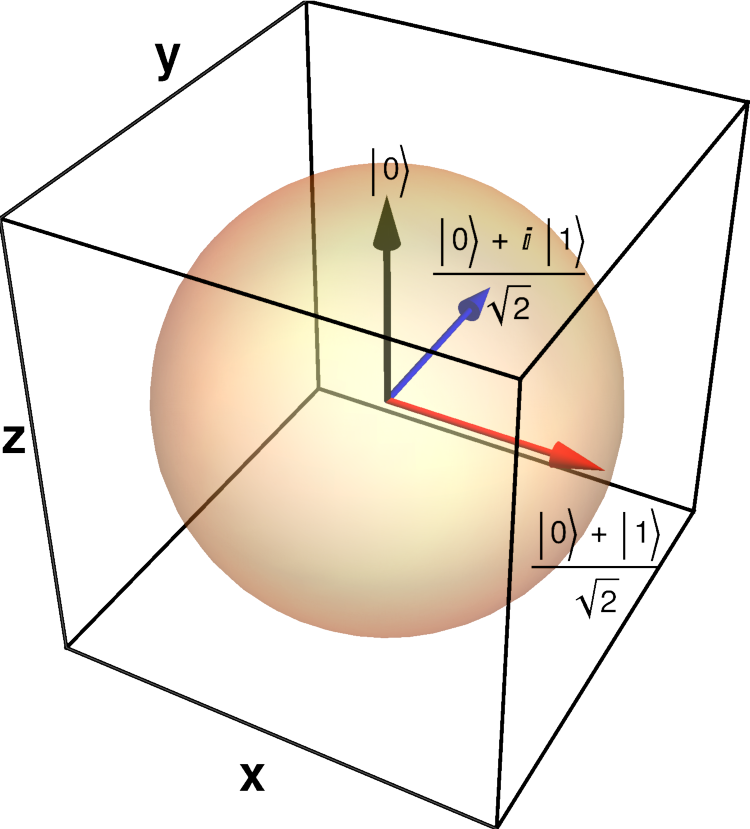
\includegraphics[width=2.5cm]{bloch_sphere2}
		& \hspace{\fill} \Large$\overset{\normalsize{R_x(\pi/3)}}{\longmapsto}$ \hspace{\fill}
		& 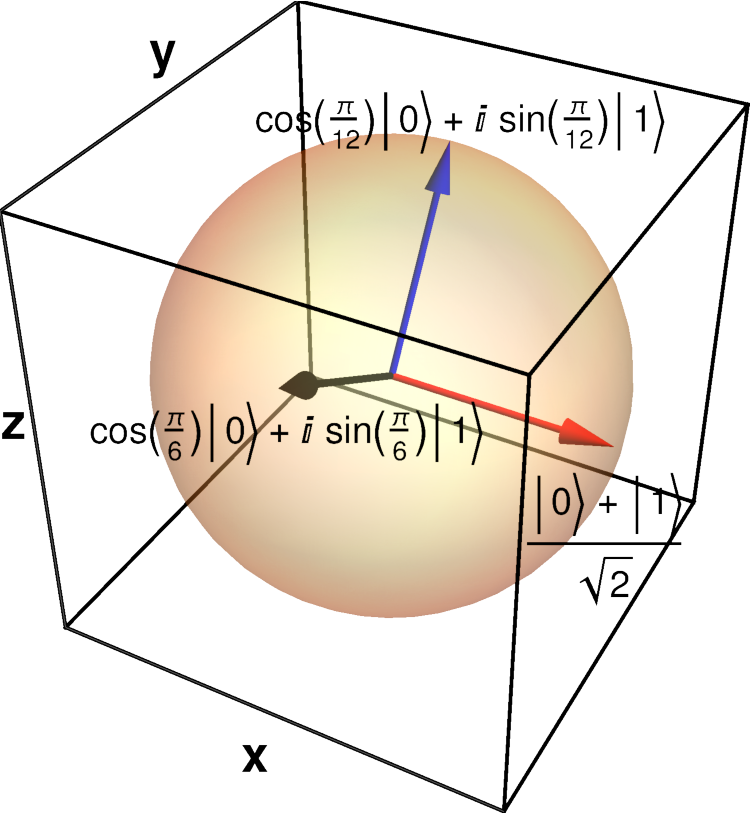
\includegraphics[width=2.5cm]{bloch_sphere_Rx_pi_medios2}
	\end{tabular}
	\end{center}
	
	Canal \textit{bit-flip}	 $\mathcal{E}$
	\begin{center}
	\begin{tabular}{m{2.5cm} m{1.8cm} m{2.5cm}}
		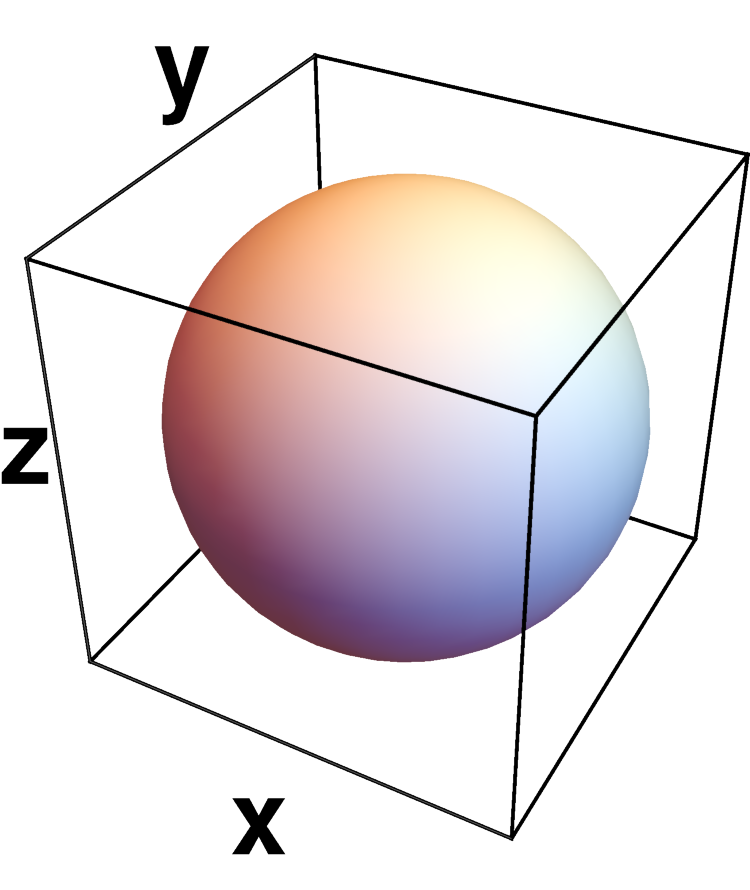
\includegraphics[width=2.5cm]{unit_sph}
		& \hspace{\fill} \Large{$\overset{\mathcal{E}}{\longmapsto}$} \hspace{\fill}
		& 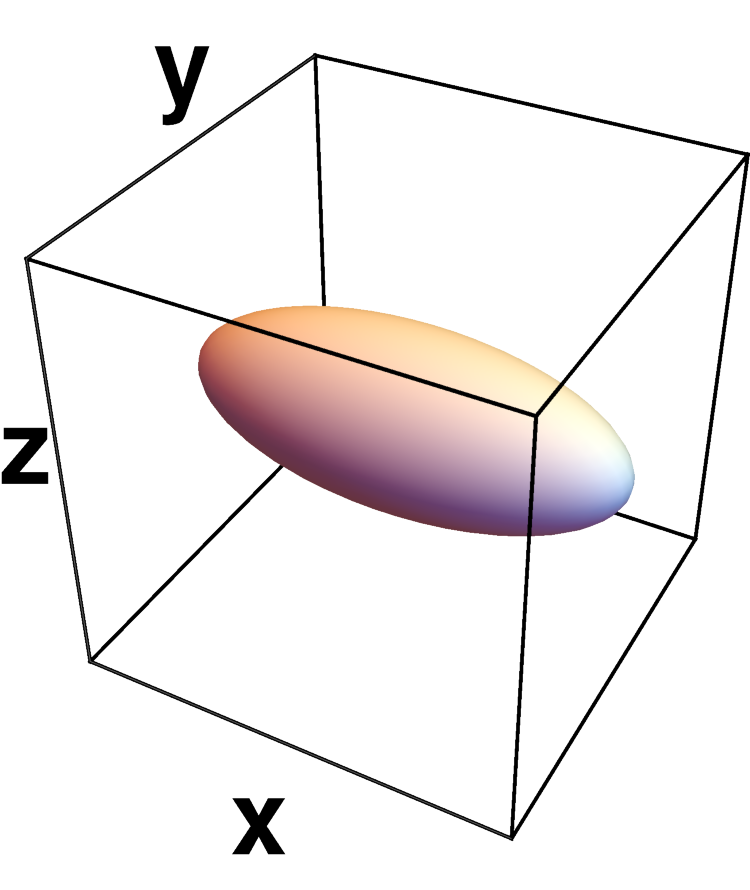
\includegraphics[width=2.5cm]{bit_flip_p0_3}
	\end{tabular}
	\end{center}
\end{frame}


% % % % % % % % % % % % % % % % % % % % % % % % % % % % % % % % % % % % % %
% Qubits
% % % % % % % % % % % % % % % % % % % % % % % % % % % % % % % % % % % % % %

\section{Operaciones PCE:}

\begin{frame}{Operaciones PCE}{Definición}
 	Una operación que borra las componentes de Pauli (operación PCE)
	es una operación lineal que transforma a las 	componentes 
	de Pauli de la matriz densidad $\rho$ de $n$ qubits como
	\begin{align*}
		r_{j_1,\ldots,j_n}\longmapsto \tau_{j_1,\ldots,j_n}\cdot r_{j_1,\ldots,j_n},
		\qquad \tau_{j_1,\ldots,j_n}=0,1.
		\end{align*} 
	Una operación PCE borra o preserva las componentes de Pauli 
	de un matriz densidad de un sistema de $n$ qubits.
\end{frame}

\begin{frame}{Figuras PCE}{Una representación geométrica}
Una operación PCE puede representarse por medio de una grilla $n-$dimensional,
cuyas posiciones se asocian con los índices de las componentes $\tau_{j_1,\ldots,
j_n}$ de una operación PCE. \vfill

\begin{itemize}
	\item 1 qubit: 
	
\resizebox{.75\textwidth}{!}{%
		\begin{minipage}{\textwidth}
		\begin{figure} % {{{
		\begin{center}
		\begin{tikzpicture}[x=0.5cm, y=0.5cm] % {{{
		\pgfmathsetmacro{\unitstep}{3.5}
		% Coordenadas   {{{
		\node at (-0.6,0.5) {(a)} ;
		\draw (0,0) rectangle (1,1); \node at (0.5,0.5) {$\tau_0$} ;
		\begin{scope}[shift={(0,-1)}]
		\draw (0,0) rectangle (1,1); \node at (0.5,0.5) {$\tau_1$} ;
		\end{scope}
		\begin{scope}[shift={(0,-2)}]
		\draw (0,0) rectangle (1,1); \node at (0.5,0.5) {$\tau_2$} ;
		\end{scope}
		\begin{scope}[shift={(0,-3)}]
		\draw (0,0) rectangle (1,1); \node at (0.5,0.5) {$\tau_3$} ;
		\end{scope} % }}}
%		\begin{scope}[shift={(1*\unitstep,0)}] % Identity {{{
%		% \begin{scope}[shift={(\unitstep*2,0)}]
%		\node at (-0.6,0.5) {(b)} ;
%		\fill[black] (0,0) rectangle (1,1);
%		\draw (0,0) rectangle (1,1);
%		\begin{scope}[shift={(0,-1)}] \fill[black] (0,0) rectangle (1,1); \end{scope}
%		\begin{scope}[shift={(0,-1)}] \draw (0,0) rectangle (1,1); \end{scope}
%		\begin{scope}[shift={(0,-2)}] \fill[black] (0,0) rectangle (1,1); \end{scope}
%		\begin{scope}[shift={(0,-2)}] \draw (0,0) rectangle (1,1); \end{scope}
%		\begin{scope}[shift={(0,-3)}] \fill[black] (0,0) rectangle (1,1); \end{scope}
%		\begin{scope}[shift={(0,-3)}] \draw (0,0) rectangle (1,1); \end{scope}
%		\end{scope} % }}}
		\begin{scope}[shift={(1*\unitstep,0)}] % Dephasing {{{
		\node at (-0.6,0.5) {(b)} ;
		\fill[black] (0,0) rectangle (1,1);
		\draw (0,0) rectangle (1,1);
		% \begin{scope}[shift={(0,-1)}] \fill[black] (0,0) rectangle (1,1); \end{scope}
		\begin{scope}[shift={(0,-1)}] \draw (0,0) rectangle (1,1); \end{scope}
		% \begin{scope}[shift={(0,-2)}] \fill[black] (0,0) rectangle (1,1); \end{scope}
		\begin{scope}[shift={(0,-2)}] \draw (0,0) rectangle (1,1); \end{scope}
		\begin{scope}[shift={(0,-3)}] \fill[black] (0,0) rectangle (1,1); \end{scope}
		\begin{scope}[shift={(0,-3)}] \draw (0,0) rectangle (1,1); \end{scope}
		\end{scope} % }}}
%		\begin{scope}[shift={(3*\unitstep,0)}] % Depolarization {{{
%		\node at (-0.6,0.5) {(d)} ;
%		\fill[black] (0,0) rectangle (1,1);
%		\draw (0,0) rectangle (1,1);
%		% \begin{scope}[shift={(0,-1)}] \fill[black] (0,0) rectangle (1,1); \end{scope}
%		\begin{scope}[shift={(0,-1)}] \draw (0,0) rectangle (1,1); \end{scope}
%		% \begin{scope}[shift={(0,-2)}] \fill[black] (0,0) rectangle (1,1); \end{scope}
%		\begin{scope}[shift={(0,-2)}] \draw (0,0) rectangle (1,1); \end{scope}
%		% \begin{scope}[shift={(0,-3)}] \fill[black] (0,0) rectangle (1,1); \end{scope}
%		\begin{scope}[shift={(0,-3)}] \draw (0,0) rectangle (1,1); \end{scope}
%		\end{scope} % }}}
		\begin{scope}[shift={(2*\unitstep,0)}] % (e) canal malo {{{
		\node at (-0.6,0.5) {(c)} ;
		\fill[black] (0,0) rectangle (1,1);
		\draw (0,0) rectangle (1,1);
		% \begin{scope}[shift={(0,-1)}] \fill[black] (0,0) rectangle (1,1); \end{scope}
		\begin{scope}[shift={(0,-1)}] \draw (0,0) rectangle (1,1); \end{scope}
		\begin{scope}[shift={(0,-2)}] \fill[black] (0,0) rectangle (1,1); \end{scope}
		\begin{scope}[shift={(0,-2)}] \draw (0,0) rectangle (1,1); \end{scope}
		\begin{scope}[shift={(0,-3)}] \fill[black] (0,0) rectangle (1,1); \end{scope}
		\begin{scope}[shift={(0,-3)}] \draw (0,0) rectangle (1,1); \end{scope}
		\end{scope} % }}}
		\end{tikzpicture} % }}}
%		
%		\vspace*{2mm}
%		\begin{tikzpicture}[x=0.5cm, y=0.5cm] % {{{
%		\pgfmathsetmacro{\unitstep}{5.8}
%		\begin{scope}[shift={(0*\unitstep,0)}] % Coordenadas {{{
%		\node at (-0.6,0.5) {(f)} ;
%		    \foreach \x in {0,1,2,3} {
%		      \foreach \y in {0,1,2,3} {
%		        \begin{scope}[shift={(\x,-\y)}] 
%		          \draw (0,0) rectangle (1,1); 
%		          \node at (0.5,0.5) {\scalebox{.6}{$\tau_{\y,\x}$}};
%		         \end{scope}
%		%         \node at (0,-\y) (input\y) {$i_\y$};
%		%         \node[block] at (2,-\y) (block\y) {$f_\y$};
%		%         \draw[->] (input\y) -- (block\y);
%		%         \draw[->] (block\y.east) -- +(0.5,0);
%		    }
%		    }
%		\end{scope} % }}}
%		\begin{scope}[shift={(1*\unitstep,0)}] % Good channel {{{
%		\node at (-0.6,0.5) {(g)} ;
%		    \foreach \x in {0,1,2,3} {
%		      \foreach \y in {0,1,2,3} {
%		        \begin{scope}[shift={(\x,-\y)}] 
%		          \draw (0,0) rectangle (1,1); 
%		%           \node at (0.5,0.5) {$\tau_{\y,\x}$};
%		         \end{scope}
%		%         \node at (0,-\y) (input\y) {$i_\y$};
%		%         \node[block] at (2,-\y) (block\y) {$f_\y$};
%		%         \draw[->] (input\y) -- (block\y);
%		%         \draw[->] (block\y.east) -- +(0.5,0);
%		    }
%		    }
%		\begin{scope}[shift={(0,-3)}] \fill[black] (0,0) rectangle (1,1); \end{scope}
%		\begin{scope}[shift={(3,-3)}] \fill[black] (0,0) rectangle (1,1); \end{scope}
%		\begin{scope}[shift={(0,0)}] \fill[black] (0,0) rectangle (1,1); \end{scope}
%		\begin{scope}[shift={(3,0)}] \fill[black] (0,0) rectangle (1,1); \end{scope}
%		\end{scope} % }}}
%%		\begin{scope}[shift={(2*\unitstep,0)}] % Good channel {{{
%%		\node at (-0.6,0.5) {(h)} ;
%%		    \foreach \x in {0,1,2,3} {
%%		      \foreach \y in {0,1,2,3} {
%%		        \begin{scope}[shift={(\x,-\y)}] 
%%		          \draw (0,0) rectangle (1,1); 
%%		%           \node at (0.5,0.5) {$\tau_{\y,\x}$};
%%		         \end{scope}
%%		%         \node at (0,-\y) (input\y) {$i_\y$};
%%		%         \node[block] at (2,-\y) (block\y) {$f_\y$};
%%		%         \draw[->] (input\y) -- (block\y);
%%		%         \draw[->] (block\y.east) -- +(0.5,0);
%%		    }
%%		    }
%%		\begin{scope}[shift={(0,0)}] \fill[black] (0,0) rectangle (1,1); \end{scope}
%%		\begin{scope}[shift={(0,-1)}] \fill[black] (0,0) rectangle (1,1); \end{scope}
%%		\begin{scope}[shift={(2,0)}] \fill[black] (0,0) rectangle (1,1); \end{scope}
%%		\begin{scope}[shift={(2,-2)}] \fill[black] (0,0) rectangle (1,1); \end{scope}
%%		\begin{scope}[shift={(2,-3)}] \fill[black] (0,0) rectangle (1,1); \end{scope}
%%		\end{scope} % }}}
%		\end{tikzpicture} % }}}
		\end{center}
		\end{figure} % }}}
		\end{minipage}}
	
	\item 2 qubits: la matriz densidad se escribe 
	$
		\rho=\sum_{i,\ j=0}^3r_{i,j}\cdot \sigma_i\otimes\sigma_j, 
	$
		
\resizebox{.75\textwidth}{!}{%
		\begin{minipage}{\textwidth}
		\begin{figure} % {{{
		\begin{center}
%		\begin{tikzpicture}[x=0.5cm, y=0.5cm] % {{{
%		\pgfmathsetmacro{\unitstep}{3.5}
%		% Coordenadas   {{{
%		\node at (-0.6,0.5) {(a)} ;
%		\draw (0,0) rectangle (1,1); \node at (0.5,0.5) {$\tau_0$} ;
%		\begin{scope}[shift={(0,-1)}]
%		\draw (0,0) rectangle (1,1); \node at (0.5,0.5) {$\tau_1$} ;
%		\end{scope}
%		\begin{scope}[shift={(0,-2)}]
%		\draw (0,0) rectangle (1,1); \node at (0.5,0.5) {$\tau_2$} ;
%		\end{scope}
%		\begin{scope}[shift={(0,-3)}]
%		\draw (0,0) rectangle (1,1); \node at (0.5,0.5) {$\tau_3$} ;
%		\end{scope} % }}}
%%		\begin{scope}[shift={(1*\unitstep,0)}] % Identity {{{
%%		% \begin{scope}[shift={(\unitstep*2,0)}]
%%		\node at (-0.6,0.5) {(b)} ;
%%		\fill[black] (0,0) rectangle (1,1);
%%		\draw (0,0) rectangle (1,1);
%%		\begin{scope}[shift={(0,-1)}] \fill[black] (0,0) rectangle (1,1); \end{scope}
%%		\begin{scope}[shift={(0,-1)}] \draw (0,0) rectangle (1,1); \end{scope}
%%		\begin{scope}[shift={(0,-2)}] \fill[black] (0,0) rectangle (1,1); \end{scope}
%%		\begin{scope}[shift={(0,-2)}] \draw (0,0) rectangle (1,1); \end{scope}
%%		\begin{scope}[shift={(0,-3)}] \fill[black] (0,0) rectangle (1,1); \end{scope}
%%		\begin{scope}[shift={(0,-3)}] \draw (0,0) rectangle (1,1); \end{scope}
%%		\end{scope} % }}}
%		\begin{scope}[shift={(1*\unitstep,0)}] % Dephasing {{{
%		\node at (-0.6,0.5) {(b)} ;
%		\fill[black] (0,0) rectangle (1,1);
%		\draw (0,0) rectangle (1,1);
%		% \begin{scope}[shift={(0,-1)}] \fill[black] (0,0) rectangle (1,1); \end{scope}
%		\begin{scope}[shift={(0,-1)}] \draw (0,0) rectangle (1,1); \end{scope}
%		% \begin{scope}[shift={(0,-2)}] \fill[black] (0,0) rectangle (1,1); \end{scope}
%		\begin{scope}[shift={(0,-2)}] \draw (0,0) rectangle (1,1); \end{scope}
%		\begin{scope}[shift={(0,-3)}] \fill[black] (0,0) rectangle (1,1); \end{scope}
%		\begin{scope}[shift={(0,-3)}] \draw (0,0) rectangle (1,1); \end{scope}
%		\end{scope} % }}}
%%		\begin{scope}[shift={(3*\unitstep,0)}] % Depolarization {{{
%%		\node at (-0.6,0.5) {(d)} ;
%%		\fill[black] (0,0) rectangle (1,1);
%%		\draw (0,0) rectangle (1,1);
%%		% \begin{scope}[shift={(0,-1)}] \fill[black] (0,0) rectangle (1,1); \end{scope}
%%		\begin{scope}[shift={(0,-1)}] \draw (0,0) rectangle (1,1); \end{scope}
%%		% \begin{scope}[shift={(0,-2)}] \fill[black] (0,0) rectangle (1,1); \end{scope}
%%		\begin{scope}[shift={(0,-2)}] \draw (0,0) rectangle (1,1); \end{scope}
%%		% \begin{scope}[shift={(0,-3)}] \fill[black] (0,0) rectangle (1,1); \end{scope}
%%		\begin{scope}[shift={(0,-3)}] \draw (0,0) rectangle (1,1); \end{scope}
%%		\end{scope} % }}}
%		\begin{scope}[shift={(2*\unitstep,0)}] % (e) canal malo {{{
%		\node at (-0.6,0.5) {(c)} ;
%		\fill[black] (0,0) rectangle (1,1);
%		\draw (0,0) rectangle (1,1);
%		% \begin{scope}[shift={(0,-1)}] \fill[black] (0,0) rectangle (1,1); \end{scope}
%		\begin{scope}[shift={(0,-1)}] \draw (0,0) rectangle (1,1); \end{scope}
%		\begin{scope}[shift={(0,-2)}] \fill[black] (0,0) rectangle (1,1); \end{scope}
%		\begin{scope}[shift={(0,-2)}] \draw (0,0) rectangle (1,1); \end{scope}
%		\begin{scope}[shift={(0,-3)}] \fill[black] (0,0) rectangle (1,1); \end{scope}
%		\begin{scope}[shift={(0,-3)}] \draw (0,0) rectangle (1,1); \end{scope}
%		\end{scope} % }}}
%		\end{tikzpicture} % }}}
%		
%		\vspace*{2mm}
		\begin{tikzpicture}[x=0.5cm, y=0.5cm] % {{{
		\pgfmathsetmacro{\unitstep}{5.8}
		\begin{scope}[shift={(0*\unitstep,0)}] % Coordenadas {{{
		\node at (-0.6,0.5) {(f)} ;
		    \foreach \x in {0,1,2,3} {
		      \foreach \y in {0,1,2,3} {
		        \begin{scope}[shift={(\x,-\y)}] 
		          \draw (0,0) rectangle (1,1); 
		          \node at (0.5,0.5) {\scalebox{.6}{$\tau_{\y,\x}$}};
		         \end{scope}
		%         \node at (0,-\y) (input\y) {$i_\y$};
		%         \node[block] at (2,-\y) (block\y) {$f_\y$};
		%         \draw[->] (input\y) -- (block\y);
		%         \draw[->] (block\y.east) -- +(0.5,0);
		    }
		    }
		\end{scope} % }}}
		\begin{scope}[shift={(1*\unitstep,0)}] % Good channel {{{
		\node at (-0.6,0.5) {(g)} ;
		    \foreach \x in {0,1,2,3} {
		      \foreach \y in {0,1,2,3} {
		        \begin{scope}[shift={(\x,-\y)}] 
		          \draw (0,0) rectangle (1,1); 
		%           \node at (0.5,0.5) {$\tau_{\y,\x}$};
		         \end{scope}
		%         \node at (0,-\y) (input\y) {$i_\y$};
		%         \node[block] at (2,-\y) (block\y) {$f_\y$};
		%         \draw[->] (input\y) -- (block\y);
		%         \draw[->] (block\y.east) -- +(0.5,0);
		    }
		    }
		\begin{scope}[shift={(0,-3)}] \fill[black] (0,0) rectangle (1,1); \end{scope}
		\begin{scope}[shift={(3,-3)}] \fill[black] (0,0) rectangle (1,1); \end{scope}
		\begin{scope}[shift={(0,0)}] \fill[black] (0,0) rectangle (1,1); \end{scope}
		\begin{scope}[shift={(3,0)}] \fill[black] (0,0) rectangle (1,1); \end{scope}
		\end{scope} % }}}
%		\begin{scope}[shift={(2*\unitstep,0)}] % Good channel {{{
%		\node at (-0.6,0.5) {(h)} ;
%		    \foreach \x in {0,1,2,3} {
%		      \foreach \y in {0,1,2,3} {
%		        \begin{scope}[shift={(\x,-\y)}] 
%		          \draw (0,0) rectangle (1,1); 
%		%           \node at (0.5,0.5) {$\tau_{\y,\x}$};
%		         \end{scope}
%		%         \node at (0,-\y) (input\y) {$i_\y$};
%		%         \node[block] at (2,-\y) (block\y) {$f_\y$};
%		%         \draw[->] (input\y) -- (block\y);
%		%         \draw[->] (block\y.east) -- +(0.5,0);
%		    }
%		    }
%		\begin{scope}[shift={(0,0)}] \fill[black] (0,0) rectangle (1,1); \end{scope}
%		\begin{scope}[shift={(0,-1)}] \fill[black] (0,0) rectangle (1,1); \end{scope}
%		\begin{scope}[shift={(2,0)}] \fill[black] (0,0) rectangle (1,1); \end{scope}
%		\begin{scope}[shift={(2,-2)}] \fill[black] (0,0) rectangle (1,1); \end{scope}
%		\begin{scope}[shift={(2,-3)}] \fill[black] (0,0) rectangle (1,1); \end{scope}
%		\end{scope} % }}}
		\end{tikzpicture} % }}}
		\end{center}
		\end{figure} % }}}
		\end{minipage}}
\end{itemize}
\end{frame}

\begin{frame}{Operaciones PCE}{El problema}
	¿Cuáles son las operaciones PCE que son operaciones físicas (canales cuánticos PCE)?\vfill
	
	Estudiamos numéricamente los casos de 1, 2 y 3 qubits.
\end{frame}

\begin{frame}[t]{Método numérico}
	\only<1>{
	\begin{columns}
		\begin{column}{0.5\textwidth}
			\begin{figure}
		\centering
		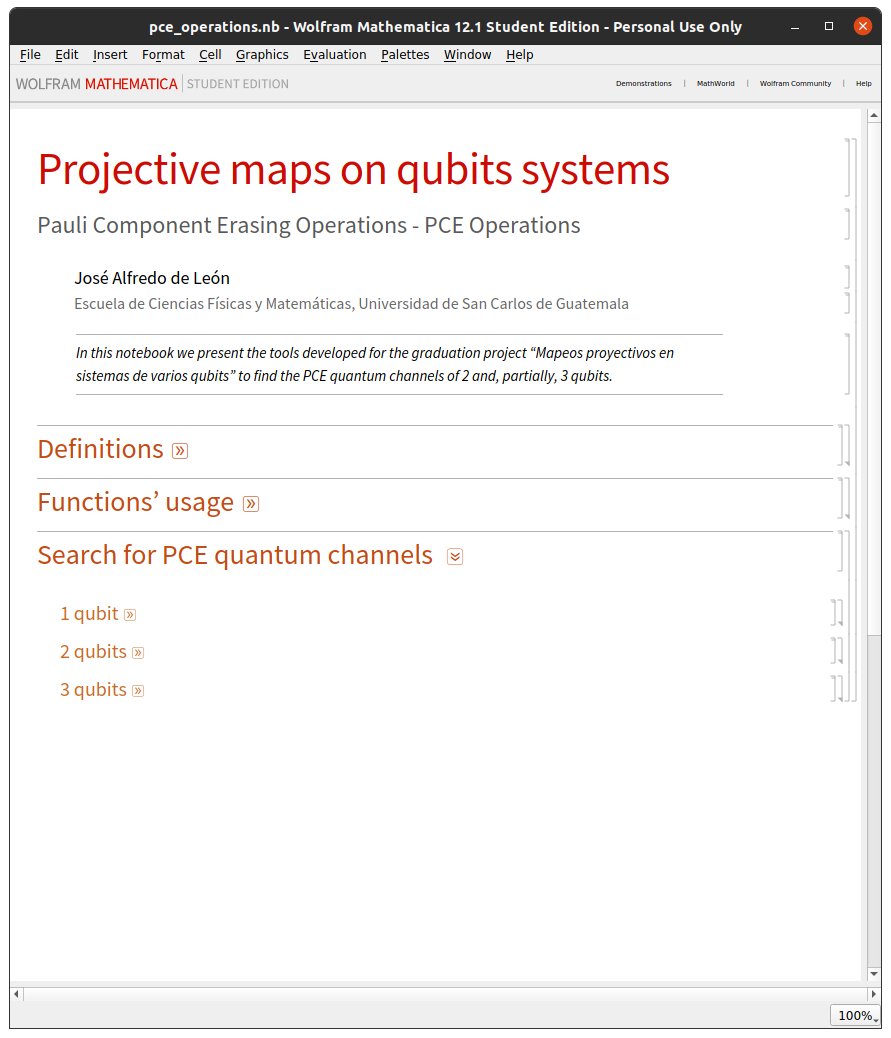
\includegraphics[width=1\textwidth]{numerico_01}
	\end{figure}		
		\end{column}
		\begin{column}{0.5\textwidth}
			\begin{figure}
		\centering
		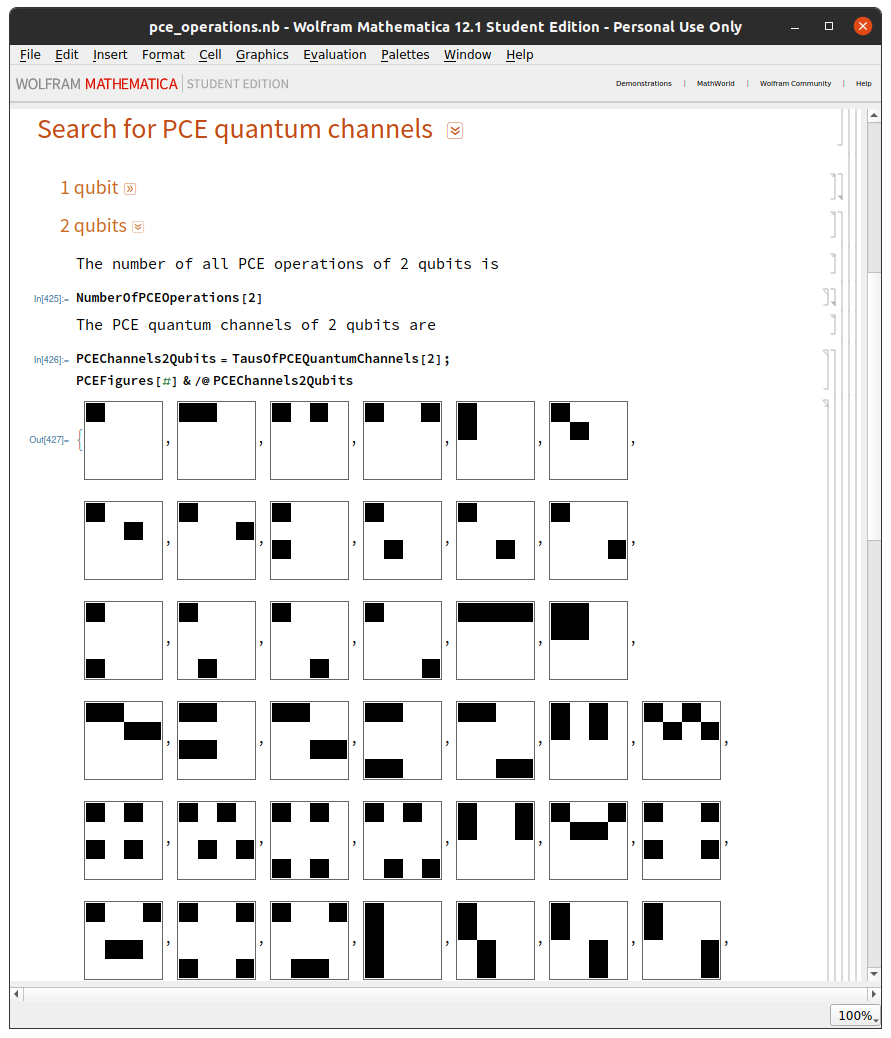
\includegraphics[width=1\textwidth]{numerico_02}
	\end{figure}		
		\end{column}
	\end{columns}		
	}
	\only<2>{
	https://github.com/deleonja/projective\_maps
	\begin{figure}
		\centering
		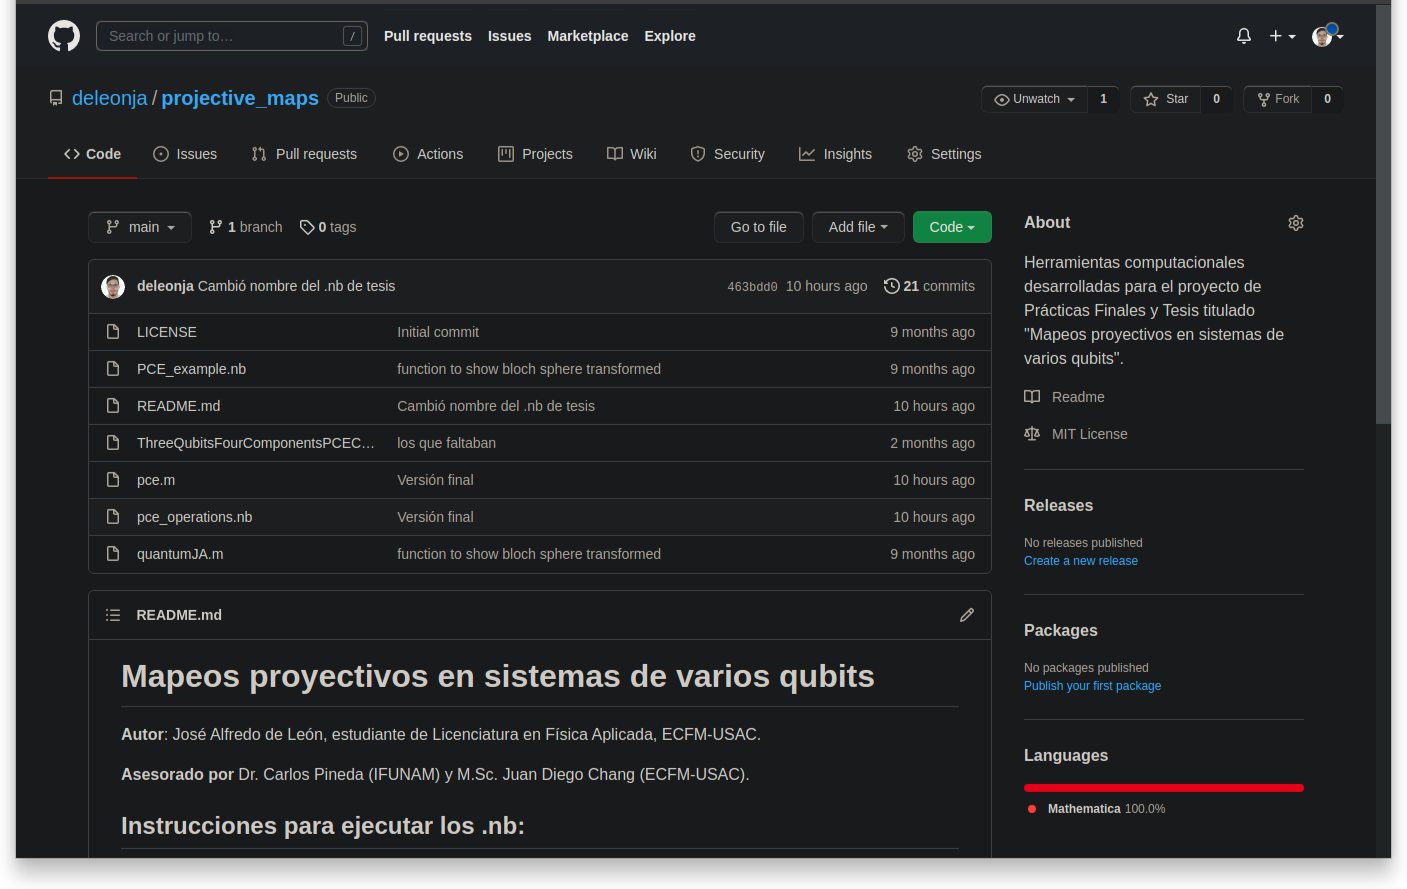
\includegraphics[width=.9\textwidth]{numerico_03}
	\end{figure}
	}
	
\end{frame}

\begin{frame}{Resultados}{Clases de equivalencia}
	Los canales cuánticos PCE pueden ordenarse en subconjuntos cuyos elementos
	son equivalente vía \vfill
	\begin{enumerate}
		\item Intercambios de partículas: un canal cuántico debe serlo para 
		cualquier configuración de partículas del sistema.
		\begin{center}
		\begin{tabular}{m{1.5cm} m{1.2cm} m{1.5cm}}
		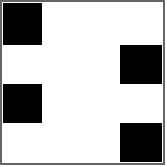
\includegraphics[height=1.5cm]{2qubits_PCE_QC_001}
		& \hspace{\fill} \Large$\longmapsto$ \hspace{\fill}
		& 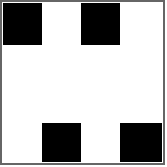
\includegraphics[height=1.5cm]{2qubits_PCE_QC_003}
		\end{tabular}
		\end{center}\vfill 
		
		\item Permutación de elementos de una base local. Por ejemplo,\newline
		para la partícula 2: 
		$\{\sigma_x,\sigma_y,\sigma_z \}\mapsto \{\sigma_z,\sigma_x,\sigma_y \}$
		
		\begin{center}
		\begin{tabular}{m{1.5cm} m{1.2cm} m{1.5cm}}
		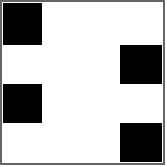
\includegraphics[height=1.5cm]{2qubits_PCE_QC_001}
		& \hspace{\fill} \Large$\longmapsto$ \hspace{\fill}
		& 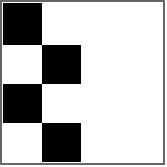
\includegraphics[height=1.5cm]{2qubits_PCE_QC_004}
		\end{tabular}
		\end{center}
	\end{enumerate}\vfill
\end{frame}

\begin{frame}{Resultados}{Regla $2^k$}
	Los canales cuánticos PCE preservan una cantidad 
	de componentes de Pauli que son potencias de dos.
	\begin{columns}[t]
		\begin{column}{0.5\textwidth}
			\begin{itemize}
				\item 1 qubit
			\end{itemize}
			\only<1>{
			Canales cuánticos PCE:
			\begin{figure}
				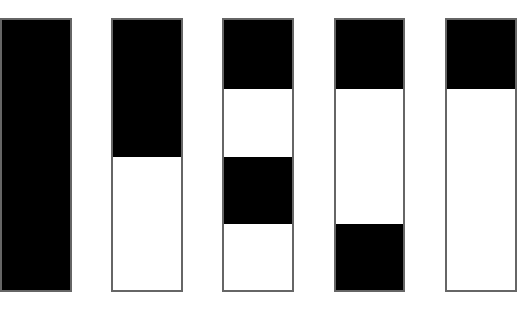
\includegraphics[height=1.4cm]{1qubit}
			\end{figure}
			Operaciones PCE no CP:
			\begin{figure}
				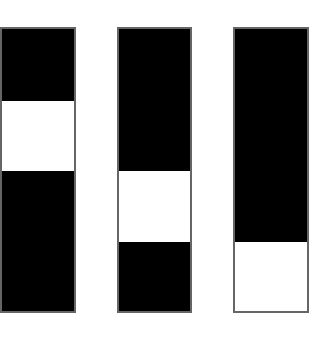
\includegraphics[height=1.6cm]{not_QC_1qubit}
			\end{figure}
			}
		\end{column} 
		\begin{column}{0.5\textwidth}		
		\begin{itemize}
		\item 2 qubits:
		\end{itemize}
		\only<1>{
		Canal cuántico PCE:
		\begin{figure}
			\centering
			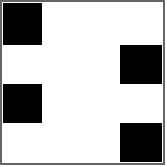
\includegraphics[height=1.5cm]{2qubits_PCE_QC_001}
		\end{figure}
		
		Operación PCE que no es CP:
		\begin{figure}
			\centering
			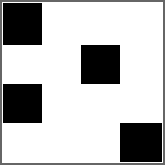
\includegraphics[height=1.5cm]{2qubits_PCE_QC_002}
		\end{figure}
		}
		\end{column}
	\end{columns}
\end{frame}

\begin{frame}{Resultados}{Regla espejo}
El número de canales cuánticos PCE en función del exponente $k$ del 
número $2^k$ de componentes de Pauli invariantes es simétrico respecto a 
$k=n$.

	\begin{figure} % {{{
	\centering
	\begin{subfigure}[b]{0.48\textwidth}
		\centering
		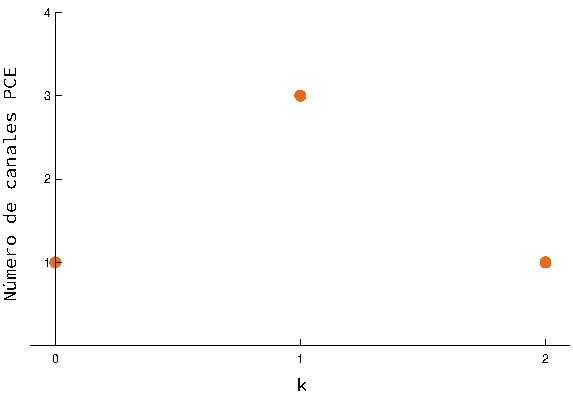
\includegraphics[width=3.7cm]{mirroring_1qubits}
		\caption{1 qubit}
		\label{fig:mirroring_1qubit}
	\end{subfigure}
	\hfill
	\begin{subfigure}[b]{0.48\textwidth}
		\centering
		\hfill 
		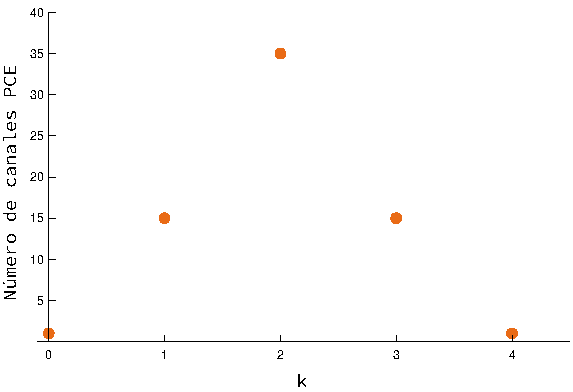
\includegraphics[width=3.7cm]{mirroring_2qubits} 
		\hfill \hfill
		\caption{2 qubits}
		\label{fig:mirroring_2qubits}
	\end{subfigure}
	\newline
	\begin{subfigure}[c]{\textwidth}
		\centering
		\hspace*{\fill}
		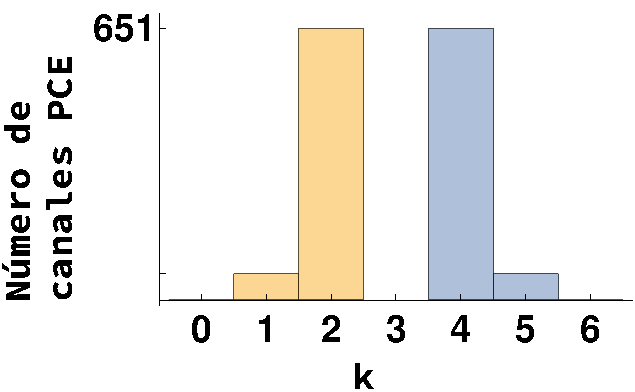
\includegraphics[width=3.7cm]{mirroring_3qubits}
		\hspace*{\fill}
		\caption{3 qubits}
		\label{fig:mirroring_3qubits}
	\end{subfigure}
	\label{fig:mirroring}
\end{figure} % }}}
\end{frame}

\begin{frame}{Canales de Ruskai}{Canales PCE, ¿un subconjunto
de otros canales de Pauli estudiados antes?}
	Encontramos que los canales PCE \alert{no son} un sobconjunto
	de los canales de Ruskai\footnote{
	M. Nathanson and M.B. Ruskai, arXiv:quant-ph/0611106 (2006)}.
	
	\begin{center}
	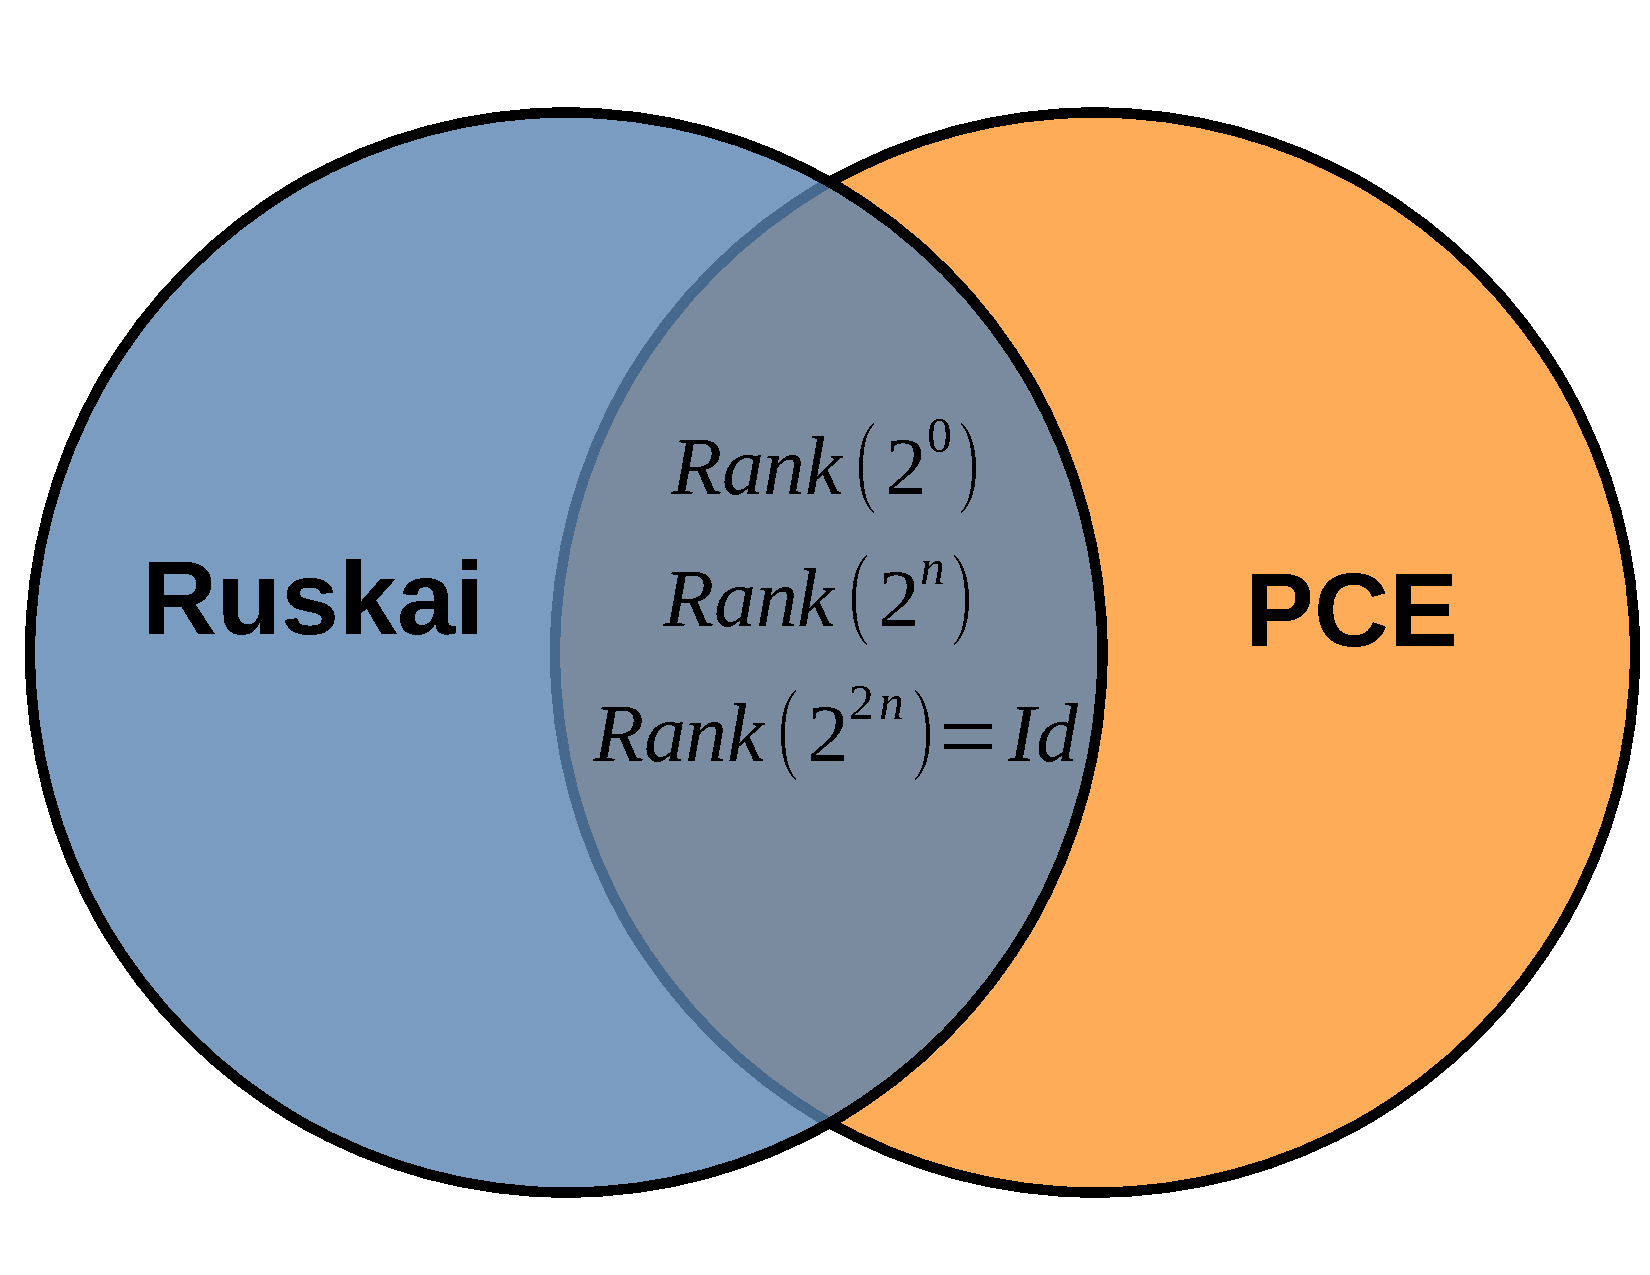
\includegraphics[width=8cm]{diagrama_venn_ruskai_y_pce}
	\end{center}
\end{frame}

\section{Conclusiones y trabajo posterior}

\begin{frame}{Conclusiones}
	\begin{itemize}
		\item Propusimos el estudio un tipo de canales cuánticos que generalizan  
		las decoherencias de una partícula de dos niveles (qubit) para sistemas de
		$n$ qubits. Exploramos numéricamente el caso de 1, 2, y, parcialmente, 3 
		qubits.
		\item Nuestros resultados (regla $2^k$, regla espejo, clases de equivalencia) 
		muestran que los canales cuánticos PCE obedecen alguna estructura matemática.
		\item Los canales cuánticos PCE no son un subconjunto de otros canales 
		de Pauli estudiados antes.
	\end{itemize}
	
%	\begin{tikzpicture}[x=1mm,y=1mm,overlay,remember picture]
%    \pgftransformshift{\pgfpointanchor{current page}{center}}
%%    \node[inner sep=0pt] (usac) at (-40,-14.5) %
%%    {
\includegraphics[height=14mm]{logos/ecfmByN}};
%%    \node[inner sep=0pt] (usac) at (39,-14.5) %
%%    {
\includegraphics[height=14mm]{logos/ifunam}};
%    \node[inner sep=0pt] (usac) at (0,-30) %
%    {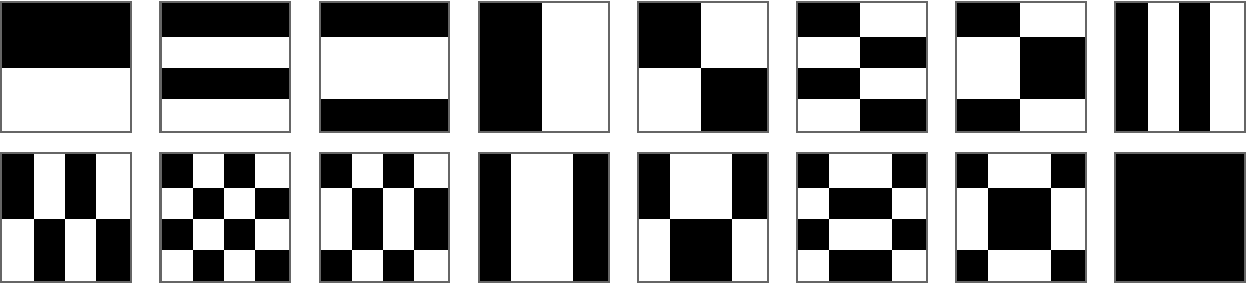
\includegraphics[height=14mm]{portada}};
%    \node[inner sep=0pt] (usac) at (50,-30) %
%    {¡gracias!};
%  \end{tikzpicture}
%	\onslide<2>{
	
%	}
\end{frame}

\begin{frame}{Trabajo posterior}
	\begin{itemize}
	\item Los resultados de este trabajo motivaron el estudio analítico de las 
	condiciones que deben satisfacer las componentes $\tau_{j_1,\ldots,j_n}$ 
	de una operación PCE para ser un canal cuántico.
	\item Encontramos que los subíndices $j_1,\ldots,j_n$ tienen una estructura 
	de espacio vectorial sobre campos de dimensión finita, estructura que explica
	las reglas $2^k$ y espejo.
	\item Encontramos que existen generadores PCE con los cuales se pueden
	construir al resto, 
		\vspace*{1mm}\begin{center}
		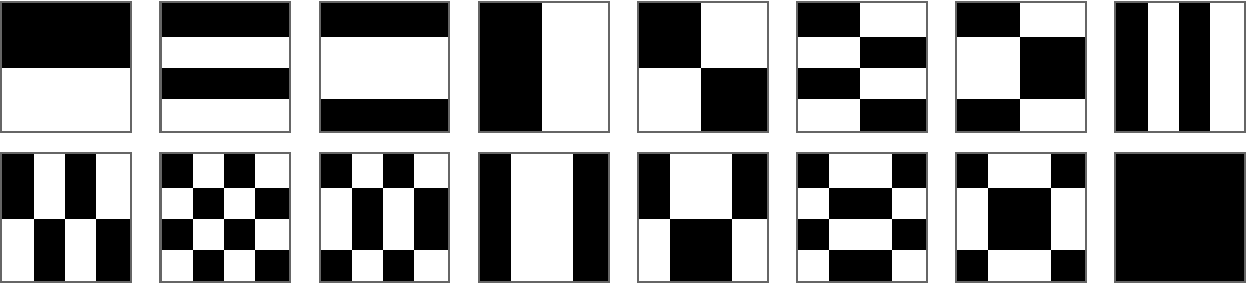
\includegraphics[height=12mm]{portada}
		\end{center}
		\item Actualmente, estamos estudiando operaciones similares a los PCE,
		de muchas partículas, pero de dimensión arbitraria (qudits). 
	\end{itemize}\vfill 
	\hfill \Large \bf ¡Muchas gracias!
\end{frame}

\end{document}
